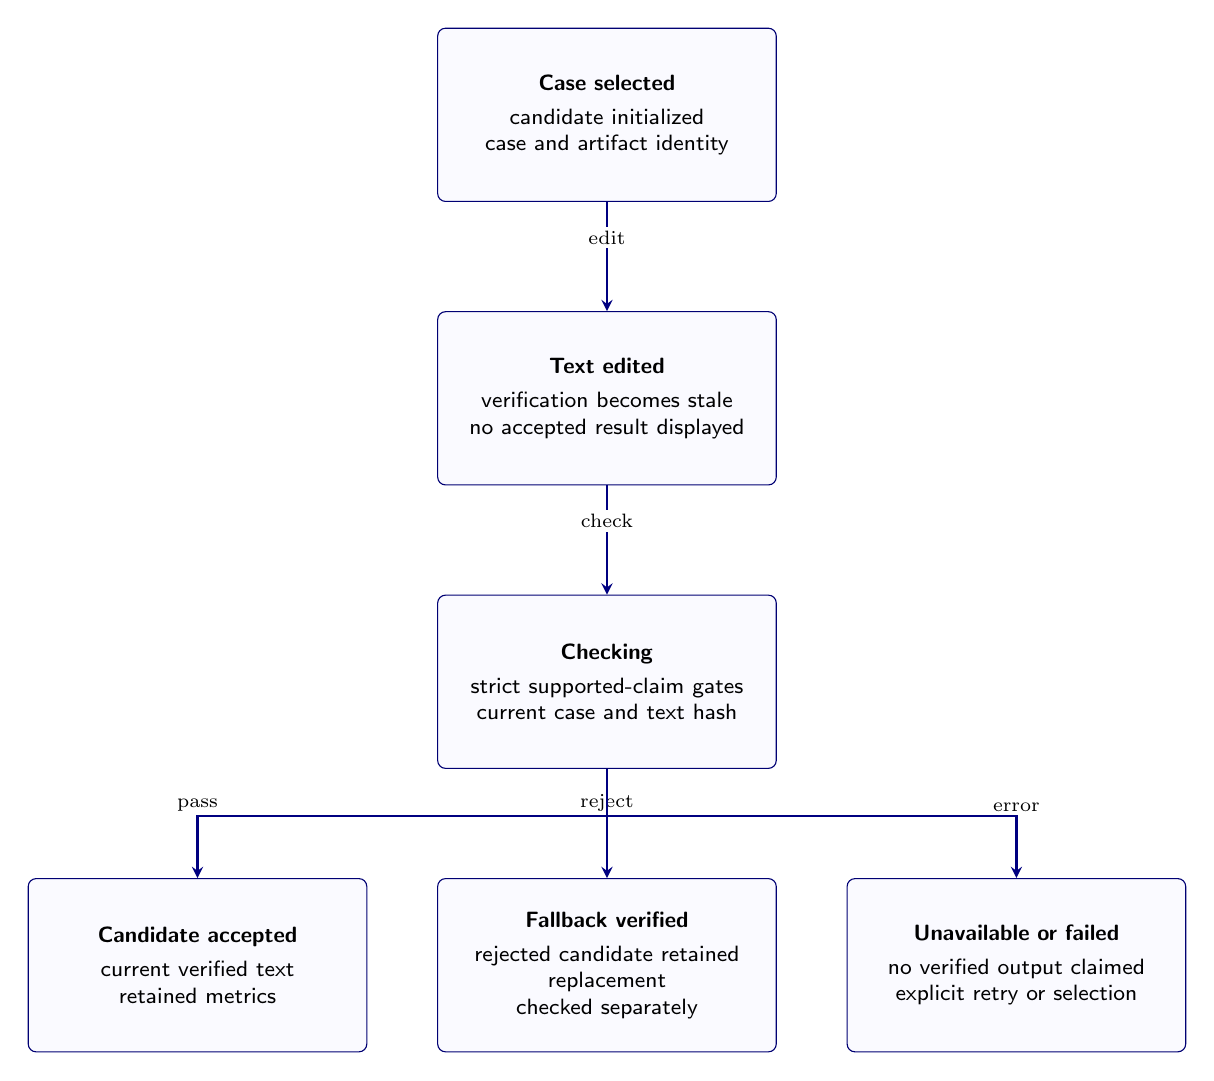
\begin{tikzpicture}[x=1mm,y=1mm,box/.style={draw=blue!45!black,fill=blue!2,rounded corners=1mm,align=center,text width=39mm,minimum height=22mm,inner sep=2mm,font=\sffamily\footnotesize},link/.style={->,>=stealth,draw=blue!50!black,thick}]
\node[box] (selected) at (75,135) {\textbf{Case selected}\\[1mm]candidate initialized\\case and artifact identity};
\node[box] (edited) at (75,99) {\textbf{Text edited}\\[1mm]verification becomes stale\\no accepted result displayed};
\node[box] (checking) at (75,63) {\textbf{Checking}\\[1mm]strict supported-claim gates\\current case and text hash};
\node[box] (accepted) at (23,27) {\textbf{Candidate accepted}\\[1mm]current verified text\\retained metrics};
\node[box] (fallback) at (75,27) {\textbf{Fallback verified}\\[1mm]rejected candidate retained\\replacement checked separately};
\node[box] (error) at (127,27) {\textbf{Unavailable or failed}\\[1mm]no verified output claimed\\explicit retry or selection};
\draw[link] (selected.south) -- ++(0,-6) -| (edited.north) node[pos=.5,above,fill=white,inner sep=.5mm,font=\scriptsize]{edit};
\draw[link] (edited.south) -- ++(0,-6) -| (checking.north) node[pos=.5,above,fill=white,inner sep=.5mm,font=\scriptsize]{check};
\draw[link] (checking.south) -- ++(0,-6) -| (accepted.north) node[pos=.5,above,fill=white,inner sep=.5mm,font=\scriptsize]{pass};
\draw[link] (checking.south) -- ++(0,-6) -| (fallback.north) node[pos=.5,above,fill=white,inner sep=.5mm,font=\scriptsize]{reject};
\draw[link] (checking.south) -- ++(0,-6) -| (error.north) node[pos=.5,above,fill=white,inner sep=.5mm,font=\scriptsize]{error};
\end{tikzpicture}
